
\section{The Picture's Size: Bounding Box and Clipping}

This section explains how a picture receives its final dimensions. The
picture's dimension is the bounding box. It is possible to restrict the
bounding box, but display graphical elements outside of the bounding box. This
is called subject of Section~\ref{sec:bb}. Another use case is to restrict both
the bounding box and the clip the graphical elements to some outer path which
is subject of Section~\ref{sec:clipping}.


\subsection{Bounding Box Restrictions}
\label{sec:bb}

Bounding box restrictions are a useful and often necessary tool if multiple
pictures need to be aligned properly. Consequently, it is often applied
together with the Alignments methods of Section~\ref{sec:pgfplots:sec:align}.

Bounding box restrictions can be achieved with several methods of \PGF{}:
%
\begin{enumerate}
    \item\label{en:overlay} The |overlay| option,
    \item The |pgfinterruptboundingbox| environment,
    \item The |\pgfresetboundingbox| command,
    \item\label{en:useasbb} The |\useasboundingbox| path,
    \item The |trim left| and |trim right| feature (which is the \emph{only}
        supported way of restricted bounding boxes and image externalization;
        at least for \textsc{pdf} output).
            \xdef\letzterwert{\the\value{enumi}}
\end{enumerate}
%
An additional item is a specific use case of \PGFPlots{}:
%
\begin{enumerate}
        \setcounter{enumi}{\letzterwert}
    \item The |hide axis| feature will exclude any axis specific stuff from
        the bounding box. See the reference for |hide axis| for
        details.\index{Bounding Box Control!hide axis}
\end{enumerate}

Note that image externalization (the |external| library) is more or less
incompatible with methods \ref{en:overlay} to \ref{en:useasbb}. The problem is
that |pdflatex| crops everything outside of the bounding box away. There are
only two safe ways to ``restrict'' bounding boxes of external |.pdf| images:
the first is the mentioned |trim left|/|trim right| feature and the second is
to use negative |\hspace| or |\vspace| commands (or options to
|\includegraphics|).

\begin{key}{/tikz/overlay}
        \index{Bounding Box Control!Excluding Image Parts}
    A special key of \PGF{} which disables bounding box updates for (parts of)
    the image. The effect is that those parts are an ``overlay'' over the
    document.

    For \PGFPlots{}, |overlay| can be useful to position legends or other axis
    descriptions outside of the axis~-- without affecting its size (and without
    affecting alignment).

    For example, one may want to include only certain parts of the axis into
    the final bounding box. This would allow horizontal alignment (centering):
    %
\begin{codeexample}[]
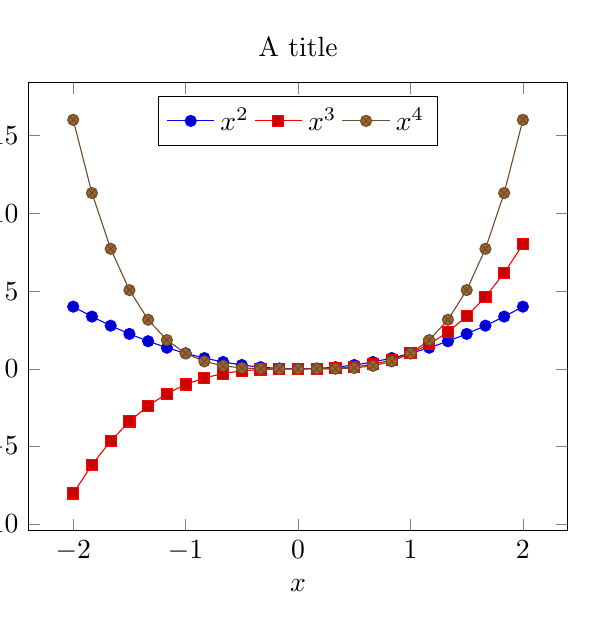
\begin{tikzpicture}
\begin{axis}[
    title=A title,
    ylabel style={overlay},
    yticklabel style={overlay},
    xlabel={$x$},
    ylabel={$y$},
    legend style={at={(0.5,0.97)},
        anchor=north,legend columns=-1},
    domain=-2:2,
]
    \addplot {x^2};
    \addplot {x^3};
    \addplot {x^4};
    \legend{$x^2$,$x^3$,$x^4$}
\end{axis}
\end{tikzpicture}
\end{codeexample}
    %
    \noindent Now, the left axis descriptions ($y$ label and $y$ ticks) stick
    out of the bounding box.

    The following example places a legend somewhere without affecting the
    bounding box.
    %
\begin{codeexample}[]
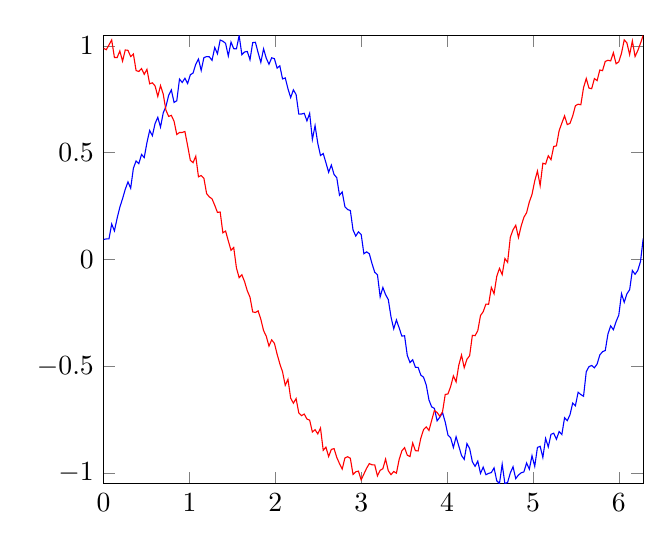
\begin{tikzpicture}
\begin{axis}[
    domain=0:6.2832,samples=200,
    legend style={
        overlay,
        at={(-0.5,0.5)},
        anchor=center},
    every axis plot post/.append style={mark=none},
    enlargelimits=false,
]
    \addplot {sin(deg(x)+3) + rand*0.05};
    \addplot {cos(deg(x)+2) + rand*0.05};
    \legend{Signal 1,Signal 2}
\end{axis}
\end{tikzpicture}
\end{codeexample}

    More information about the |overlay| option can be found in the \PGF{}
    manual~\cite{tikz}.
\end{key}

\begin{command}{\pgfresetboundingbox}
    This command of \pgfname{} resets the bounding box of the current picture.
    The computation starts from scratch afterwards, allowing to compute a
    user-defined bounding box.
    %
\begin{codeexample}[]
\setlength{\fboxsep}{0pt}%
\fbox{%
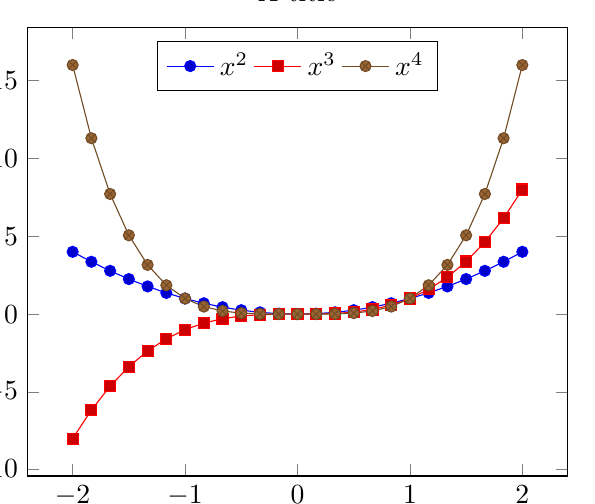
\begin{tikzpicture}
    \begin{axis}[
        title=A title,
        xlabel={$x$},
        ylabel={$y$},
        legend style={at={(0.5,0.97)},
            anchor=north,legend columns=-1},
        domain=-2:2,
    ]
        \addplot {x^2};
        \addplot {x^3};
        \addplot {x^4};
        \legend{$x^2$,$x^3$,$x^4$}
    \end{axis}

    \pgfresetboundingbox
    \path
              (current axis.south west)
    rectangle (current axis.north east);
\end{tikzpicture}%
}
\end{codeexample}
    The example draws a normal picture, containing an axis. Afterwards, it
    throws the bounding box away and creates a new one based on the
    |current axis| node and its anchors.
\end{command}

\begin{environment}{{pgfinterruptboundingbox}}
    \index{Bounding Box Control}
    \index{Bounding Box Control!pgfinterruptboundingbox}

{
        \pgfmanualpdflabel{\textbackslash useasboundingbox}{}
    Yet another approach with the same effect is shown below: the bounding box
    is interrupted manually, and resumed afterwards.
    %
\begin{codeexample}[]
\setlength{\fboxsep}{0pt}%
\fbox{%
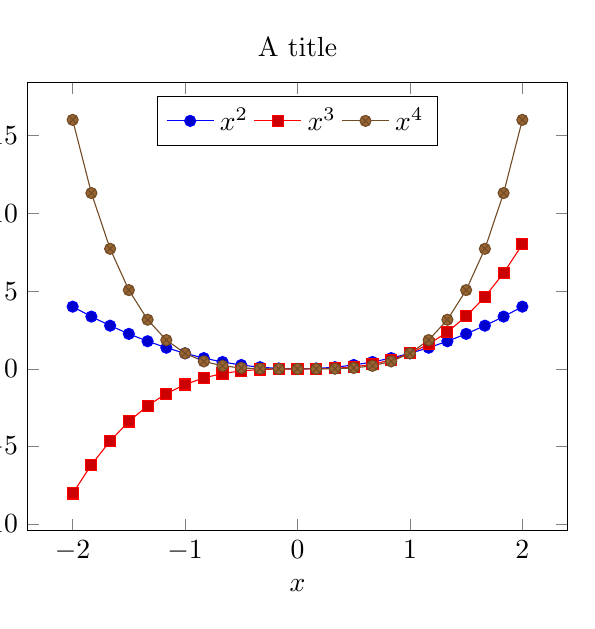
\begin{tikzpicture}
  \begin{pgfinterruptboundingbox}
    \begin{axis}[
        title=A title,
        xlabel={$x$},
        ylabel={$y$},
        legend style={at={(0.5,0.97)},
            anchor=north,legend columns=-1},
        domain=-2:2,
    ]
        \addplot {x^2};
        \addplot {x^3};
        \addplot {x^4};
        \legend{$x^2$,$x^3$,$x^4$}
    \end{axis}
  \end{pgfinterruptboundingbox}

    \useasboundingbox
                  (current axis.below south west)
        rectangle (current axis.above north east);
\end{tikzpicture}%
}
\end{codeexample}
}
    %
    The |pgfinterruptboundingbox| environment does not include its content into
    the image's bounding box, and |\useasboundingbox| sets the pictures
    bounding box to the following argument (see~\cite{tikz}).
\end{environment}

\begin{keylist}{%
    /tikz/trim left=\marg{$x$-coordinate or point} (default 0pt),
    /tikz/trim right=\marg{$x$-coordinate or point}%
}
    These
    %\todosp{why is the first value green and the second black?}%
    % -> some magic with Till Tantaus coloring styles: one has a
    %    default whereas the other doesn't
    two keys allow to reduce the size of the bounding box.

    The |trim left| key expects either a single $x$-coordinate like |1cm| or a
    point like |(current axis.west)|. If a point is provided, is uses only the
    $x$-coordinate of that point. Then, the left end of the bounding box is set
    to the resulting $x$-coordinate and everything left of it is outside of the
    bounding box.

    The |trim right| key has the same effect, only for the right end of the
    bounding box.

    More detailed documentation can be found in the \Tikz{} manual.
\end{keylist}

\begin{stylekey}{/tikz/trim axis left}
    A style with value |trim left=(current axis.south west)|.

    The style needs to be provided as argument to
    |\begin{tikzpicture}[trim axis left]|. It expects (at least) one
    \PGFPlots{} environment in the picture. The effect is to trim everything
    which is left of the last axis' anchor |south west| (i.e.\@ everything left
    of the left axis boundary).
\end{stylekey}

\begin{stylekey}{/tikz/trim axis right}
    A style with value |trim right=(current axis.south east)|.

    It works similarly to |trim axis left|: the effect is that everything right
    of the right axis line of the last axis environment is truncated from the
    bounding box.
\end{stylekey}

\begin{stylekey}{/tikz/trim axis group left}
    A style which has the same effect as |trim axis left|, but is tailored for
    the |groupplots| library.

    It has the value |trim left=(group c1r1.south west)|.

    The style needs to be provided as argument to
    |\begin{tikzpicture}[trim axis group left]|. It expects (at least) one
    |groupplot| environment in the picture. The effect is to trim everything
    which is left of the first group axis' anchor |south west| (i.e.\@
    everything left of the left axis boundary).
\end{stylekey}

\begin{stylekey}{/tikz/trim axis group right}
    A style which has the same effect as |trim axis right|, but is tailored for
    the |groupplots| library.

    It works similarly to |trim axis group left|: the effect is that everything
    right of the rightmost axis in a group plot (the last element of the
    |groupplot| environment) is truncated from the bounding box.
\end{stylekey}


\subsection{Clipping}
\label{sec:clipping}

Clipping influences both the picture size and the visible output in contrast to
bounding box restrictions which reduce the picture's final size while keeping
the same graphical output.

Typically, \PGFPlots{} uses the path for a boxed axis as clip path. However,
clipping has some special features and fine-tuning keys which are explained in
this section.

\begin{pgfplotskey}{clip=\mchoice{true,false} (initially true)}
        \index{Bounding Box Control!clip}
    Controls whether any paths inside of an axis shall be clipped.

    This is in effect even if |hide axis=true|.

    Note that a clip path can contribute to the picture's bounding box.
    Starting with |compat=1.8|, \PGFPlots{} applies intelligence to separate
    the responsibilities clipping and bounding box control, see
    |clip bounding box| and its choices. As of |compat=1.8|, a clip path can be
    in effect although the bounding box is considerably smaller than the clip
    path. This is typically what one expects if the clip path is invisible.

    The clip path is generated using |\pgfplotspathaxisoutline|, i.e.\@ it is
    the path induced by boxed axis lines. For a three-dimensional plot, only
    the outer axis lines are used. A plot with centered axis lines uses the
    outer axis lines as well.
\end{pgfplotskey}

\begin{pgfplotskey}{clip marker paths=\mchoice{true,false} (initially false)}
    The initial choice |clip marker paths=false| causes markers to be drawn
    \emph{after} the clipped region. Only their positions will be clipped.

    As a consequence, markers will be drawn completely, or not at all. The
    value |clip marker paths=true| is here for backwards compatibility: it does
    not introduce special marker treatment, so markers may be drawn partially
    if they are close to the clipping boundary.\footnote{Please note that
    clipped marker paths may be slightly faster during \TeX{} compilation.}

    This key has no effect if |clip=false|.

    Note that clip marker paths also affects the sequence in which plots and
    their markers are drawn on top of each other. See also the related key
    |clip mode|.
\end{pgfplotskey}

\begin{pgfplotskey}{%
    clip bounding box=\mchoice{default tikz,upper bound} (initially controlled by compat key)%
}
    Controls how the path generated by |clip=true| contributes to the bounding
    box. This has a consequence for |axis lines|$\neq$|box|, in particular, for
    |hide axis|: if the value is \declareandlabel{default tikz}, hiding (parts
    of) the axis will not reduce the bounding box because the clip path is as
    large as before. The value \declareandlabel{upper bound} allows to reduce
    the bounding box also in case of |hide axis|.

    More precisely, the choice \declaretext{default tikz} installs the clip
    path induced by the axis as ordinary \tikzname{} path (see
    |\pgfplotspathaxisoutline|). That means its bounding box essentially
    contributes to the picture's bounding box, irrespective of the size of
    contained paths.

    The choice \declaretext{upper bound} allows to \emph{reduce} the picture's
    bounding box to what is actually shown: if the picture only contains
    graphical elements which are completely within the bounding box of
    |\pgfplotspathaxisoutline|, the bounding box is made up of those contained
    elements. If the contained elements are actually larger than the bounding
    box of |\pgfplotspathaxisoutline|, they are clipped to the outline's path
    (``upper bound''). The latter case ensures that parts of the graphics which
    are excluded by |clip| are not counted for the bounding box.

    Keep in mind that |hide axis| is independent of |clip=true|: the clip path
    might still be in effect even though the axis outline is invisible.

    This key is irrelevant if |clip=false|. In addition, it has no effect for
    |axis lines=box| since the |box| path is made up from
    |\pgfplotspathaxisoutline|. It has an effect for |hide axis=true| or for
    choices of |axis lines| in which parts of the axis are empty.

    This key is controlled by the |compat| level. Its default is
    |default tikz|. Since |compat=1.8|, it is set to |upper bound|.

    The key has no effect if |clip=false|.
\end{pgfplotskey}

\begin{pgfplotskey}{clip mode=\mchoice{global,individual} (initially global)}
    This key controls how \PGFPlots{} implements the |clip=true| feature (which
    is on by default). Its primary motivation is control where markers are
    placed: are markers on top of everything else (choice |global|) or are they
    overdrawn by following plots (choice |individual|)?

    The choice \declaretext{global} tells \PGFPlots{} to install one single
    clip path for the complete picture.\footnote{The choice \texttt{clip
    mode=global} was the only supported clipping mechanism up to and including
    version 1.5.} In order to avoid clipped marker paths, any markers are
    processed after the clip path has been closed, i.e.\@ on a separate layer
    (see |clip marker paths|). An unexpected side effect is that marks are on
    top of plots, even if the plots have been added after the markers.

    The choice \declaretext{individual} instructs \PGFPlots{} to install a
    separate clip path for \emph{every} |\addplot| command. Consequently, the
    plot will be clipped. But most importantly, its markers will be drawn
    immediately after the clip path has been deactivated.

    An unexpected side effect of |clip mode=individual| is that
    %
    \begin{enumerate}
        \item the resulting PDF will be slightly larger due to the repeated
            paths,
        \item custom drawing instruction like |\node| or |\draw| need to be
            clipped \emph{manually}: use
            %
\begin{codeexample}[]
\begin{tikzpicture}
\begin{axis}[
    clip mode=individual,
]
    \addplot+ [samples=3] {x^2};

    \begin{scope}
        \clip \pgfextra{\pgfplotspathaxisoutline};
        \draw (-20,15) -- (20,15);
        \draw (-20,20) -- (20,20);
    \end{scope}

    \addplot+ [samples=2] {x};
\end{axis}
\end{tikzpicture}
\end{codeexample}
            %
            \noindent to install a custom clip path around your |\draw|
            instructions for such a use case. Here, the path instruction
            |\pgfplotspathaxisoutline| results in a path of the axis outline,
            i.e.\@ the path which is used for the background paths or for
            clipping. Since it is a basic level macro, it needs to be
            encapsulated by |\pgfextra|.
    \end{enumerate}

    Note that |clip marker paths| can lead to the same result as
    |clip mode=individual| if the plot does not reach the boundaries.
\end{pgfplotskey}
